\documentclass[10pt, conference]{IEEEtran}
\ifCLASSINFOpdf
\else
\fi
\usepackage{amssymb}
\usepackage[cmex10]{amsmath}
\usepackage{algorithmic}
\usepackage{array}
\usepackage{url}
\usepackage{multirow}
\usepackage{multicol}
\usepackage{graphicx}
\usepackage{graphicx}
\usepackage{mdwtab}
\usepackage{textgreek}
\usepackage[ruled,vlined]{algorithm2e}
\usepackage{graphicx}
\usepackage{epstopdf}
\usepackage{caption}
\newcommand{\figwidth}{0.75\linewidth}
\newcommand{\figwidthsmall}{0.5\linewidth}
\newcommand{\figwidtha}{0.7\linewidth}
\newcommand{\figwidthb}{0.80\linewidth}
\newcommand{\figwidthdouble}{0.5\linewidth}
\newcommand{\figwidthtriple}{0.32\linewidth}
\def\figref#1{Fig.~\ref{#1}}
\def\secref#1{Section~\ref{#1}}
\def\tabref#1{Table~\ref{#1}}
\DeclareMathOperator{\trace}{trace}
\graphicspath{ {./fig/} }

\begin{document}

\onecolumn
\tableofcontents
\listoffigures
\listoftables
\twocolumn
\clearpage

\pagenumbering{arabic} % resets the page number and sets the style to arabic
\setcounter{page}{1}  % resets the page counter to 1
\pagestyle{plain}

\title{Enhancing the Dynamic Adaptive Replication Strategy for P2P Systems Using Time-Based Decaying Function}

% author names and affiliations
\author{\IEEEauthorblockN{Abhiteja Mandava, Sai Kiran Madupu, Sai Santhosh Yamsani, Vineeth Reddy Govind} \\
 \IEEEauthorblockA{Computer Engineering Department\\
 San Jos\'{e} State University (SJSU)\\
 San Jos\'{e}, CA, USA \\
 Email: \{abhiteja.mandava, saikiran.madupu, saisanthosh.yamsani, vineethreddy.govind\}@sjsu.edu}
 }

% make the title area
\maketitle
\IEEEpeerreviewmaketitle
\begin{abstract}
Availability is one of the most important aspects of a peer-to-peer (P2P) network. To maintain the high availability of data, replication strategies are used to create multiple copies of the data file. As the number of replicas increases, the availability and performance of the system will improve. For each node in the network, the data replication decision is made based on a) which file to replicate, b) when to replicate, and c) where to place the replicated file. Most replication strategies use fixed threshold values on a node's current load of requests as criteria to replicate. However, this approach may lead to over-replication as it does not utilize timing information. For example, Dynamic Adaptive Replication Strategy (DARS) is one of the strategies that can achieve high availability and create a relatively small number of replicas. It addresses the problem of when to replicate the file by recognizing potential overload with overheating similarity (i.e., node's proximity to overload threshold) and finds the optimal placement node using fuzzy clustering analysis. However, when deciding which files need to be replicated, DARS simply picks the file with the highest number of accesses, as it is more likely to cause an overload (i.e., exceed the node’s available bandwidth) without considering the timestamps of those requests. Thus, DARS may falsely pick a file that was frequently used in the past but miss a file that is more frequently used now, leading to suboptimal performance. To overcome this problem, we propose to use a Time-Based Decaying Function (TBDF) to rank the candidate files for replication. TBDF takes the temporal locality of file accesses into consideration by utilizing timestamps of requests. It also reduces the weight and relevance of file accesses as time passes. To evaluate our approach, we developed a highly efficient event-driven P2P network simulator and configured it to several network topologies. The result shows that our approach achieves a 37.65\% improvement in node availability, 2.14\% available bandwidth, and 3.35\% latency compared to DARS.
\end{abstract}

\begin{IEEEkeywords}
file replication, peer-to-peer networks, decentralized file storage, weight-based replica selection.
\end{IEEEkeywords}

\section{Introduction}\label{sec:introduction}


The exponential rise in digital content generation and consumption has led to an increased need for efficient and scalable data management systems. Peer-to-peer (P2P) \cite{sun_2018_dars} networks have emerged as an effective solution due to their decentralized nature, capacity for data distribution, and fault tolerance. However, a crucial factor that determines the efficiency and reliability of a P2P network is the availability of data. To ensure high availability and performance, P2P networks utilize replication strategies that create multiple copies of data files across various nodes in the network. A key challenge in these replication strategies is deciding which file to replicate, when to replicate it, and where to place the replicated file. The majority of replication strategies utilize fixed threshold values on a node's current load of requests as criteria for replication, which could potentially lead to over-replication and waste of resources.

Dynamic Adaptive Replica Strategy (DARS) \cite{sun_2018_dars} addresses the problems of replica creation time and replica placement. First, the strategy obtains the replica creation opportune moment based on the node's overheating similarity (the probability that a node changes into an overloaded node). Then, it applies the fuzzy clustering analysis \cite{ling_2007_fuzzy} to find the optimal placement node. However, it selects the replication files based on the access frequency and does not consider the timestamps of the requests for the file. When deciding the set of files that need replica, DARS gets the access amount of files from an array that stores them in descending order. They assume that the files with the highest number of requests are more likely to cause an overloaded (i.e., exceed the node's available bandwidth) node without considering the timestamps of their requests. However, we found that this is not the optimal solution, as timing information also plays a critical role in determining the future access pattern. To further understand the problem, consider that files $F\textsubscript{1}$ and $F\textsubscript{2}$ have 50 and 30 hits, respectively, and most of the requests for $F\textsubscript{1}$ were made long ago, while requests made for $F\textsubscript{2}$ were recent. Therefore, it is likely that $F\textsubscript{2}$ will be re-accessed shortly compared to $F\textsubscript{1}$. This means that the timing of requests plays a vital role in determining the probability of future access. Therefore, the P2P data replication algorithms that do not use timestamp information could lead to sub-optimal system performance. 

Temporal locality is the natural tendency of applications to repeatedly utilize the same data objects while running over a period of time. This is the underlying idea of caching mechanisms and outlines a clear direction for an efficient data management strategy. This implies that the files accessed recently are likely to be reaccessed. Therefore, it is recommended that more importance be given to a recently accessed file than a file that was accessed a long time ago, along with the number of times it has been accessed. In the above example scenario, requests for F1 should be less important than requests for file F2. This can be accomplished by assigning weights that diminish over time. This can be achieved using a Time-Based Decaying Function (TBDF) \cite{gill_2016_a}. TBDF uses the concept of exponential decay function, which decays the value of TBDF with the passage of time.

To address the limitation of DARS, we propose a novel data replication strategy that incorporates the Time-Based Decaying Function (TBDF). TBDF assigns weights to files based not only on their access frequency but also on the recency of access. By leveraging the concept of temporal locality, where the likelihood of reaccessing a file decreases over time, our strategy prioritizes recently accessed files over those accessed in the past. This approach ensures that the replication process considers both the frequency and timing of file access, resulting in more efficient and optimal data replication.

To evaluate the effectiveness of our proposed approach, we have developed a highly efficient event-driven P2P network simulator. This simulator provides a realistic environment for conducting comprehensive experiments and evaluating the performance of the replication strategy under various network topologies. It accurately models the interactions between network nodes, allowing us to measure key performance metrics such as node availability, available bandwidth, and latency.

The rest of the paper is organized as follows: In Section II, we review the related work and state of the art in the field of data replication in P2P networks. Section III presents the design of our proposed approach, focusing on the file selection process. In Section IV, we describe the implementation details. Section V outlines our evaluation methodology, including trace data, event-driven simulation, network topology, evaluation metrics, and experimental setup. Section VI presents the evaluation results, followed by a discussion of the findings and future work in Section VII. Finally, we conclude the paper in Section VIII.

% A node becomes overloaded when the number of requests exceeds the node's available bandwidth, making it unable to respond to the requests quickly. Data replication is an effective method to overcome the problem of node overloading, as it distributes the load across multiple peers \cite{shen_2008_ead} and results in lower latency. As a file that is most frequently requested can quickly exhaust the node's bandwidth, the conventional replication strategies copy this file to other nodes. These strategies use a predetermined fixed threshold for replica creation based on metrics like node load and bandwidth \cite{shen_2008_ead}. When the node reaches predefined conditions, the hot file (a file that causes the node to become overloaded) on the overloaded node creates a replica and stores the replica on another node. However, these traditional solutions \cite{amjad_2012_a} may cause a few issues \cite{shakarami_2021_data} under high-load situations.

% The first risk pertains to the replica creation time. When the node reaches or surpasses the predefined threshold, these methods create a replica. However, the node is already overloaded at this point, thereby increasing the number of overload nodes. As a result, finding the optimal time for replica creation is crucial. Another problem might occur during the replica placement process.  When an overloaded node makes a replica and stores it on another node, the placement node may also become overloaded, resulting in the aggregate effect of being overloaded. Therefore, selecting the best node to store the replica must be carefully considered. Lastly, there could also be a risk while choosing the replication file. The conventional methods replicate the files with the highest number of requests. However, the file may no longer be frequently accessed in the future, thus leading to stale replicas. Hence, it is essential to strategize which file to replicate.

\section{Background}\label{sec:background}
Peer-to-Peer (P2P) systems revolutionize traditional client-server models by enabling decentralized networks where participants, known as peers, collaboratively contribute their computing resources to provide services and share data. Unlike centralized architectures, P2P systems distribute the workload and data storage across multiple peers, leading to enhanced scalability, fault tolerance, and improved performance. P2P networks have gained significant popularity and find application in various domains, including file sharing, content delivery, real-time collaboration, and distributed computing.

In P2P systems, each peer acts as both a client and a server, allowing direct communication and data sharing among the peers without the need for a central server. Peers contribute their computing power, storage capacity, and network bandwidth, making the system dynamically scalable and self-organizing. The decentralized nature of P2P networks eliminates the reliance on a single point of failure, resulting in higher robustness and resilience to failures.

The main contribution of this project is as follows:

\begin{enumerate}
\item Proposal and Design of a Novel Replication Strategy: We propose and design a novel replication strategy specifically tailored for Peer-to-Peer (P2P) networks. Our strategy utilizes a time-based decaying function to effectively improve load balancing, alleviate network bandwidth congestion, and enhance overall resource usage efficiency in P2P networks.

\item Design and Implementation of an Event-driven P2P Network Simulator: We implemented and thoroughly evaluated our enhanced replication strategy using a meticulously crafted event-driven P2P network simulator. Our custom simulator outperformed traditional cycle-based simulators, enabling more efficient and accurate simulation of P2P network behavior.

\item Performance Evaluation Results: Through comprehensive evaluation, we demonstrate the effectiveness of our proposed strategy. The evaluation results reveal significant improvements over the existing Dynamic Adaptive Replica Strategy (DARS). Specifically, our strategy achieves a remarkable 30\% reduction in overheat duration, a substantial 37.65\% reduction in unavailable duration, an impressive 3.35\% lower latency, and a notable 2.14\% reduction in average bandwidth consumption when compared to DARS.
\end{enumerate}

By achieving these objectives, we aim to contribute to the field of P2P systems by developing a more dynamic and efficient replication strategy that adapts to changing access patterns and improves the overall performance of P2P networks.


In the following sections, we will elaborate on the design and implementation of the enhanced replication strategy, along with the details of the event-driven P2P network simulator. We will also present the evaluation methodology and discuss the results of our experiments, highlighting the advantages and effectiveness of the proposed approach.

\subsection{Related Work}
Milani et al. \cite{ALAMIMILANI2016229} discussed several approaches that allow their associated replication strategies to be adjusted at run time according to user behavior and network topology changes. Lin et al. proposed two QoS-aware Data Replication (QADR) algorithms in cloud computing systems to support the quality of service (QoS) requirements of applications \cite{lin_dynamic}. The first algorithm adopts the intuitive idea of high-QoS first-replication (HQFR) but cannot minimize the data replication cost and the number of QoS-violated data replicas. The second algorithm uses the well-known minimum-cost maximum-flow (MCMF) problem to produce an optimal solution in polynomial time, although more computational time is required. Node combination techniques are proposed to reduce the data replication time, and simulation experiments are conducted to demonstrate the effectiveness of the algorithms. Boru et al. proposed a data replication technique focusing on energy efficiency and bandwidth consumption \cite{boru_energy}. In addition to improved quality of service, the results from the mathematical model and simulations reveal potential tradeoffs between performance and energy efficiency. They can be used to guide the design of future replication solutions.

Traditional file replication strategies often cause high storage consumption. To achieve better load balancing and data reliability needs, the paper \cite{sun_2019_rrsd} presents a file replication approach - data reliability and reducing storage consumption in a dynamic Cloud-P2P (RRSD). To accomplish its objective, RRSD applies the techniques of ”multiple replica placement” and ”redundant replica elimination.” Sun et al. claim that the system’s performance increases as more replicas are added \cite{sun_2009_dynamic}. However, most replication strategies techniques create an excess number of replicas which causes overhead for consistency and storage maintenance. Therefore, the authors presented a dynamic minimum access cost-based replication (MAC replication) approach \cite{sun_2009_dynamic}. The MAC replication strategy considers the access frequency, network connection state, and average response time. The most popular files are chosen first, and the resource that needs to be replicated is determined by calculating the average response time for each popular file.

In order to better assess the effectiveness of a replication strategy, it is necessary to have \cite{chang_2008_a} well-defined metrics and frameworks that can evaluate the performance of the system under high-load conditions. In paper [11], a framework for studying the replica placement reliability is studied by proposing a metric called Mean Time To Data Loss (MTTDL). MTTDL indicates how long, on average, the system can last after being loaded with data objects before losing the first data object in the system permanently. Huang et al. \cite{huang2014modeling} presented an analysis of the reliability of data nodes and the corresponding network links and proposed a reliability model for cloud storage systems. The paper first introduces the relationships among the access reliability, the replica numbers and the user access frequency, the reliability of data service and the trigger mechanism of replica generation, and the storage node selection. Then, the paper proposes the replica distribution algorithm and the replica deletion algorithm.

These works emphasized a single dimension of data replication, like evaluation strategy, reducing additional storage overhead, QoS, and energy efficiency. Meanwhile, our proposed solution focuses on improving file replica placement, file creation time, and file selection in the P2P network.

\subsection{State of the art}
Sun et al. proposed DARS (Dynamic adaptive replication strategy) \cite{sun_2009_dynamic}, which suggests that node overload is caused by the number of requests it receives in a given time. It assumes this is mainly due to the number of requests for local files and the number of requests the node forwards. This strategy proposes that a node can reduce the risk of overload by creating a replica before it becomes too hot. However, it should not create replicas indiscriminately, as this may increase unnecessary replicas. It is suggested that replicas should be created when a node's load is close to reaching the overload threshold, which is described as overheating similarity. The membership function of overheating similarity determines the proximity of the current node state to the overload state. To obtain the replica creation opportune moment, DARS describes the relationship between the request, node load, overheating similarity, and membership function of overheating similarity. It is proposed that a node create replicas when the load reaches a pre-defined similarity range to reduce the overload probability. This range, which consists of the floor and ceiling values of the overheating similarity, is used to determine the opportune moment for replica creation. This measure is especially effective in high-load conditions.


In this work, we build upon the foundation laid by Dynamic Adaptive Replication Strategy (DARS) paper \cite{sun_2018_dars}. The DARS paper provides a comprehensive description of the calculations and algorithms involved in the file selection process. For brevity, we refer readers to the original work for detailed explanations of these calculations. Our proposed strategy follows the same steps outlined in DARS:

\begin{enumerate}
\item Each storage layer node $HC_i$ calculates its load factor.
\item If the load factor $q_i$ exceeds the pre-hot threshold $\theta$, it indicates the possibility of node overload, prompting the initiation of the replication process.
\item When the overheating probability $A(q_i)$ falls within the similarity range $[\alpha, \epsilon)$, the node selects the files causing the overload.
\item The array $A_{HC}$ is obtained, where files are ordered based on their decay factor.
\item The neighborhood set of nodes $U_{HC}$ is determined using fuzzy clustering analysis.
\item The overheating probability and node degree of all nodes in the neighborhood set are calculated.
\item The node with the highest node degree and lowest overheating probability (with precedence given to overheating probability) is selected.
\item The files in $A_{HC}$ are stored in the optimal placement node P.
\end{enumerate}

By leveraging the existing calculations and algorithms from DARS, we ensure consistency and comparability in our evaluation. The details and justifications behind these calculations can be found in the original work by Sun et al. \cite{sun_2018_dars}.

\section{Design}\label{sec:design}

The design of our proposed replication strategy in peer-to-peer (P2P) networks incorporates a file selection process that leverages a time-based decaying function (TBDF). The TBDF plays a crucial role in prioritizing files based on their temporal locality, taking into account both the access frequency and timing information.

At each node in the network, the TBDF tracks the access amount of files and captures the timing information of file access events. The access amount of each file is continuously monitored, and at regular intervals, the TBDF value is calculated using an exponential decay function. This value is then multiplied by the access amount, resulting in an adjusted weight that reflects the importance or priority of each file.

\begin{equation}
W_{i} = F_{i} \times \sum_{k=0}^n e^{(t_{f_i^k}-t)/\beta}
\end{equation}

Where:
\begin{align*}
W_{i} &\text{ is the adjusted weight of the file } f_{i}, \\
F_{i} &\text{ is the access frequency of the file } f_{i}, \\
n &\text{ is the number of number of access of the file} f_{i}, \\
t_{f_i^k} &\text{ represents the } k\text{-th access timestamp of the file } f_{i}, \\
t &\text{ denotes the current timestamp } t, \\
\beta &\text{ is a constant.}
\end{align*}

Once the weights are calculated for all files, the replication strategy selects files with higher weights as candidates for replication. These files are deemed more important or likely to be accessed in the future, and replicating them can help improve availability and reduce access latency. The use of a TBDF in file selection enhances the replication strategy's ability to adapt to changing access patterns over time. By considering the temporal locality of file access, the strategy can prioritize files that are more relevant and timely for replication, resulting in improved performance and efficiency of the overall system.



\begin{center}
\begin{figure}[htbp]
  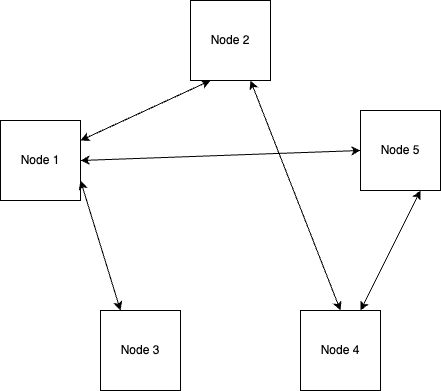
\includegraphics[width=0.45\textwidth]
  {project/fig/topology.png}
  \caption{Partial mesh network topology configuration with 5 nodes used in the the simulation.}
  \label{fig:topology}
\end{figure}
\end{center}

\section{Implementation}\label{sec:implementation}
The implementation of the replication strategy in a Peer-to-Peer (P2P) network requires careful consideration given the autonomous nature of the nodes in the network. In our setup, each node operates as an independent process and manages its own file system. These nodes interact and coordinate their actions through inter-process communication (IPC), specifically using shared memory. This approach allows the nodes to exchange information efficiently and maintain a consistent view of the network's state.

The decision for file replication, called the replica creation opportune moment, is a critical part of the strategy. Each node continuously monitors its workload, determining a metric known as the overheating similarity, which estimates the likelihood of the node becoming overloaded. When the overheating similarity reaches a certain threshold (defined by parameters α and ε), the node initiates the replication process to distribute its load.

Upon the arrival of new file requests at a node, each request is timestamped and placed in a priority queue. The positioning in this queue is determined by weights that are calculated using a Time-Based Decay Function (TBDF). TBDF provides a mechanism to decrease the value or importance of older file requests over time. This means recent file requests are prioritized over older ones, helping to ensure that the system is responsive to changes in file access patterns and that frequently and recently accessed files are replicated in a timely manner.

When a node determines that it needs to create a replica, it selects the file from the top of its priority queue, i.e., the file with the highest TBDF weight. Instead of communicating with a centralized gateway or other nodes, it relies on the shared memory to make a decision about where the new replica should be hosted. This shared memory holds the periodically updated overheating similarity for all nodes, providing a snapshot of the load situation across the network.

Based on the information from the shared memory, the node autonomously selects the most suitable peer to host the new replica. Factors like the potential host node's current load and overheating similarity are considered in this decision. This approach allows the system to adapt in real-time to changes in node workloads and network conditions, providing an efficient, decentralized mechanism for load balancing and file replication.

Once the replication process is complete, the node updates its own file system to reflect the new replica. It then uses shared memory to notify all other nodes about the replication and the new file location. This notification allows other nodes to route future file requests effectively, ensuring the new replica helps alleviate network load.

This implementation, therefore, provides a dynamic, self-regulating replication strategy that effectively prevents node overload, balances load across the P2P network, and optimizes system performance. Each node's independent processes and file systems, along with the shared memory IPC for efficient communication, contribute to this robust and responsive strategy.
\section{Evaluation Methodology}\label{sec:evaluation}
In this section, we describe the evaluation methodology used to assess the performance and effectiveness of our proposed replication strategy in P2P networks. We leverage trace data from the G4 Yahoo network flows dataset to drive our simulation and evaluation. This dataset captures real-world communication patterns between end-users and Yahoo servers, allowing us to recreate realistic network scenarios and accurately model the request patterns and communication dynamics observed in a P2P environment.

To evaluate the replication strategy, we employ an event-driven simulation approach. This approach offers several advantages for capturing the dynamics and interactions within P2P networks. It enables the modeling of asynchronous and concurrent interactions between network nodes, allowing each node to independently process events based on its own state and the current network conditions. By simulating real-world scenarios where peers interact in a decentralized manner, we obtain more accurate and realistic results.
\subsection{Trace Data}
Trace data plays a crucial role in evaluating the performance and effectiveness of replication strategies in P2P networks. Realistic trace data provides insights into actual communication patterns and can be used to generate realistic workloads for simulation and analysis.

In this research, we utilize trace data from the G4 Yahoo network flows dataset to drive our simulation and evaluation. The G4 Yahoo dataset contains a vast amount of communication patterns between end-users and Yahoo servers, capturing the dynamics of real-world network traffic. Each record within the dataset includes essential information such as timestamps, source IP addresses, and destination IP addresses, and request headers. Using the source IP address we obtain the location information such as latitude and longitude and we mapped the destination IP address to a file id. The request headers contain the information of whether the request is a read or write. These details allow us to recreate realistic network scenarios and accurately model the request patterns and communication dynamics observed in a P2P environment. 

By leveraging trace data, we can ensure that the simulation environment reflects the characteristics and complexities of real-world scenarios. This enables us to evaluate the proposed replication strategy under realistic workloads and assess its performance, efficiency, and scalability in a manner that aligns with actual network behaviors. 
\subsection{Event-driven simulation}
The event-driven simulation approach offers several advantages for evaluating the replication strategy in our research project. Firstly, it enables the modeling of asynchronous and concurrent interactions between network nodes, capturing the distributed nature of P2P networks and the interactions between peers. This approach allows each node to independently process events based on its own state and the current network conditions. It facilitates the simulation of real-world scenarios where peers interact in a decentralized manner, leading to more accurate and realistic results.

Secondly, the event-driven approach provides flexibility in modeling complex network dynamics and workload patterns. The simulation environment can be configured to replicate various network topologies and different workload intensities. This flexibility allows for evaluating the replication strategy under different network conditions and workload scenarios, providing a comprehensive understanding of its performance across a wide range of scenarios. It enables the identification of potential bottlenecks, resource limitations, and performance issues that may arise in practical P2P networks.

The key components of the simulation environment include the Request Generator, Messaging Queue, Execution Engine/Network Gateway, and Network Nodes. The Request Generator generates file request events based on real-time trace data, simulating the behavior of users and their interactions with the network. The Messaging Queue acts as a central hub for communication within the simulated network, ensuring proper message routing and synchronization among the nodes. The Execution Engine/Network Gateway serves as the bridge between the request generator and the P2P network, consuming file request events from the messaging queue and forwarding them to the relevant network nodes. The Network Nodes represent individual peers in the P2P network, processing file request events according to the replication strategy being evaluated. These components collectively create an event-driven simulation environment that closely emulates the behavior of a real-world P2P network, allowing for the evaluation of the replication strategy in a controlled and accurate manner.

By utilizing the event-driven simulation approach, our evaluation methodology provides valuable insights into the performance and effectiveness of the proposed replication strategy. It captures the dynamic and distributed nature of P2P networks, enabling the assessment of key performance metrics such as file access latency, average bandwidth utilization, overload duration, and unavailable duration. The simulation results help to evaluate the strategy's impact on load balancing, resource utilization, and overall network performance. The event-driven simulation approach ensures a comprehensive evaluation of the replication strategy's performance under different scenarios, facilitating the identification of strengths, weaknesses, and areas for improvement.

\begin{figure}[htbp]
    \centering
    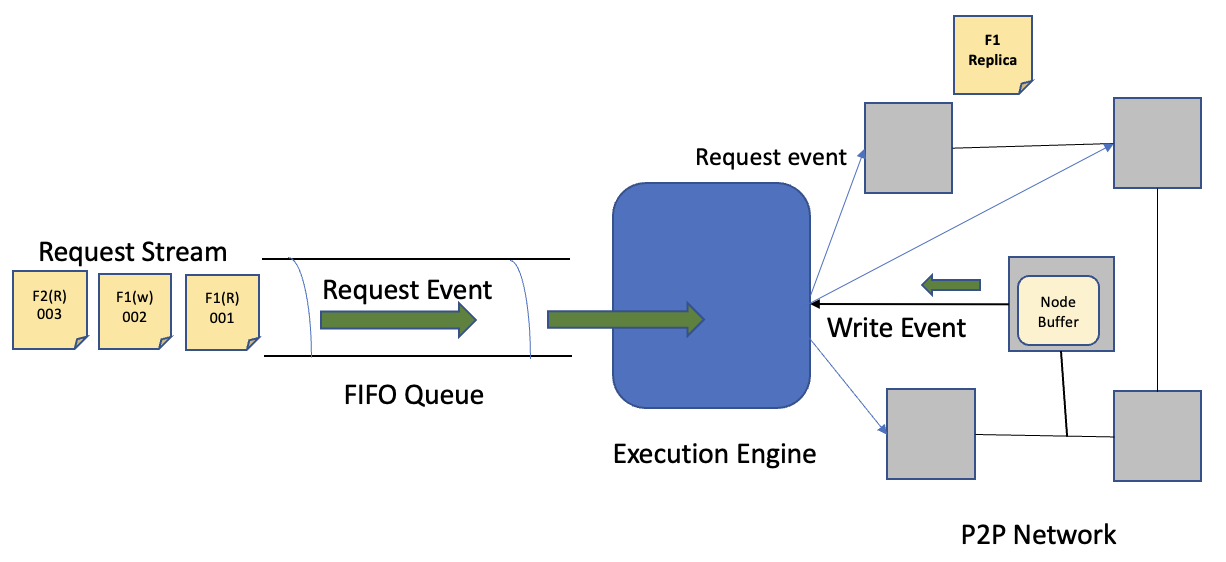
\includegraphics[width=0.45\textwidth]
    {project/fig/architecture.png}
    \caption{Components of the event-driven P2P network simulator.}
    \label{fig:architecture}
\end{figure}

\subsection{Network Topology}
In this research, we have evaluated the proposed replication strategy by conducting simulations using various network topologies. These topologies include fully connected, ring, and mesh structures, which allow us to assess the strategy's performance and effectiveness under different network configurations.

\noindent \textbf{Fully Connected.} In this topology, every node is directly connected to every other node in the network. This configuration enables efficient and direct communication between nodes, facilitating rapid file replication and dissemination. The fully connected topology provides a comprehensive assessment of the replication strategy's performance in a highly interconnected network.

\noindent \textbf{Ring.} In the ring topology, nodes are connected in a circular manner, with each node having exactly two neighbors. This configuration forms a closed loop, allowing messages and replicated files to be passed from one node to its adjacent neighbors. The ring topology is useful for evaluating the replication strategy's behavior and efficiency in a structured and cyclic network.

\noindent \textbf{Mesh.} The mesh topology consists of interconnected nodes where each node is connected to multiple other nodes in a non-linear fashion. This configuration allows for a high degree of redundancy and fault tolerance in the network. The mesh topology provides insights into how the replication strategy handles complex network structures and copes with potential network disruptions or node failures.

By utilizing these different network topologies, we can assess the replication strategy's performance and behavior under diverse scenarios. Each topology presents unique challenges and opportunities for evaluating the strategy's ability to replicate files, maintain consistency, and achieve load balancing across the network. Throughout the evaluation process, we collect and analyze various metrics, such as file access latency, average bandwidth utilization, and system availability, to gain a comprehensive understanding of the replication strategy's performance in each network topology. This analysis enables us to draw meaningful conclusions about the strategy's effectiveness and its potential applicability in real-world P2P networks with varying network structures and configurations.

\subsection{Evaluation Metrics}\label{subsec:metrics}
The evaluation of the proposed replication strategy requires well-defined metrics to assess its performance and effectiveness. In this research, several key evaluation metrics are considered to measure various aspects of the system's performance. These metrics provide insights into the impact of the replication strategy on access latency, bandwidth utilization, and node status.

\noindent \textbf{File Access Latency.} This metric measures the duration of a file request, including the network round-trip time and file processing time. Lower access latency indicates improved responsiveness and faster access to requested files.

\noindent \textbf{Average Bandwidth Utilization.} This metric quantifies the percentage of bandwidth used by each node in the network. It reflects the efficiency of bandwidth allocation and distribution across the network. Lower average bandwidth utilization suggests a more balanced load distribution and optimal resource utilization.

\noindent \textbf{Overheat.} This metric captures the duration during which a node's bandwidth usage exceeds 70\% of its maximum capacity. Overheating can lead to increased latency and decreased performance. Monitoring the overheat duration helps assess the effectiveness of the replication strategy in managing node load and preventing excessive resource consumption.

\noindent \textbf{Unavailable.} This metric measures the duration during which a node's bandwidth usage reaches 100\% of its maximum capacity. When a node is unavailable, it cannot serve any new requests, leading to service disruption and potential performance degradation. Tracking the unavailable duration provides insights into the system's availability and the effectiveness of the replication strategy in avoiding resource exhaustion.


\noindent \textbf{Average Overheating Similarity.} This metric measures the degree to which nodes approach the threshold of becoming overloaded. It quantifies the similarity between a node's current state and the threshold of overload. A higher average overheating similarity indicates a higher probability of nodes becoming overloaded. This metric helps evaluate the effectiveness of the replication strategy in managing node load and preventing overload. By analyzing the average overheating similarity, we can assess the strategy's ability to maintain a balanced and stable network environment.

\subsection{Experimental Setup}\label{subsec:setup}
To evaluate the performance of the proposed replication strategy, we conducted a series of experiments using the event-driven network simulator described in Section \ref{sec:design}. This section provides details on the experimental setup, including the network topologies, workload generation, and replication strategy configurations.

We designed and implemented three different network topologies to simulate various P2P network scenarios: fully connected, ring, and mesh topologies. These topologies represent different levels of connectivity and allow us to examine the performance of the replication strategy in different network structures.
We configured the replication strategy parameters, including the threshold for replica creation, decay function parameters, and replica placement criteria. These configurations were set based on empirical analysis and previous studies in the field.


We employed the evaluation metrics discussed in Section \ref{subsec:metrics} to measure the performance of the replication strategy. These metrics allowed us to assess key aspects such as access latency, bandwidth utilization, node status, and average overheating similarity. By analyzing these metrics, we gained insights into the effectiveness and efficiency of the proposed replication strategy.
During the experiments, we executed multiple runs for each network topology. We carefully controlled the variables and ensured consistent experimental conditions. Data was collected and analyzed using statistical methods to compare the performance of the proposed replication strategy against existing approaches.

The experimental setup provided a robust and controlled environment to evaluate the replication strategy's performance and effectiveness. The combination of different network topologies, realistic workload, and well-defined evaluation metrics allowed us to obtain meaningful results and draw valid conclusions about the proposed approach.


\section{Evaluation Results}\label{sec:results}


% Please add the following required packages to your document preamble:
% \usepackage{multirow}
% \usepackage{graphicx}
\begin{table*}[htbp]
\centering
\caption{Percentage of time each node spent in different state using the proposed replication strategy vs. DARS. The last row shows the relative percentage changes comparing the same state between the two approaches.}
\label{tab:results}
\resizebox{\textwidth}{!}{%
\begin{tabular}{ccccccc}

\hline
\vspace{5pt}
\multirow{2}{*}{\textbf{Node}} & \multicolumn{3}{c}{\textbf{Proposed Strategy}} & \multicolumn{3}{c}{\textbf{DARS}} \\ \cline{2-7} 
\vspace{5pt}
 &
  \textit{\textbf{\begin{tabular}[c]{@{}c@{}}Normal \\ Condition\end{tabular}}} &
  \textit{\textbf{Overheat Condition}} &
  \textit{\textbf{\begin{tabular}[c]{@{}c@{}}Not\\ Available\end{tabular}}} &
  \textit{\textbf{\begin{tabular}[c]{@{}c@{}}Normal \\ Condition\end{tabular}}} &
  \textit{\textbf{Overheat Condition}} &
  \textbf{\begin{tabular}[c]{@{}c@{}}Not\\ Available\end{tabular}} \\ 
  \hline
\vspace{1pt}
Node 1                         & 96.58         & 1.71           & 1.71          & 98.68     & 1.32      & 0         \\
\vspace{1pt}
Node 2                         & 99.36         & 0.43           & 0.21          & 91.74     & 3.03      & 5.23      \\
\vspace{1pt}
Node 3                         & 95.74         & 2.35           & 1.91          & 98.93     & 1.07      & 0         \\
\vspace{1pt}
Node 4                         & 100           & 0              & 0             & 100       & 0         & 0         \\
\vspace{1pt}
Node 5                         & 97.02         & 1.49           & 1.49          & 93.60     & 3.05      & 3.50      \\ \hline
\vspace{2pt}
Average                        & 97.74         & 1.19           & 1.06          & 96.6      & 1.70      & 1.70      \\ \hline
\vspace{2pt}
Change\%                       & +1.01\%       & -30.00\%       & -37.65\%      & -1.17\%   & +42.86\%  & +60.38\%  \\ \hline
\end{tabular}%
}
\end{table*}

\begin{figure}[htbp]
    \centering
    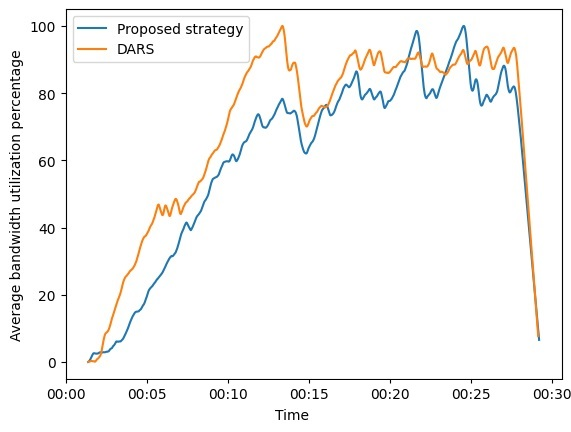
\includegraphics[width=0.45\textwidth]
    {project/fig/bandwidth.jpg}
    \caption{Average bandwidth utilization of all the nodes in the network using the proposed replication strategy vs. DARS. The x-axis shows the simulated time in the environment.}
    \label{fig:bandwidth}
\end{figure}

\begin{figure}[htbp]
    \centering
    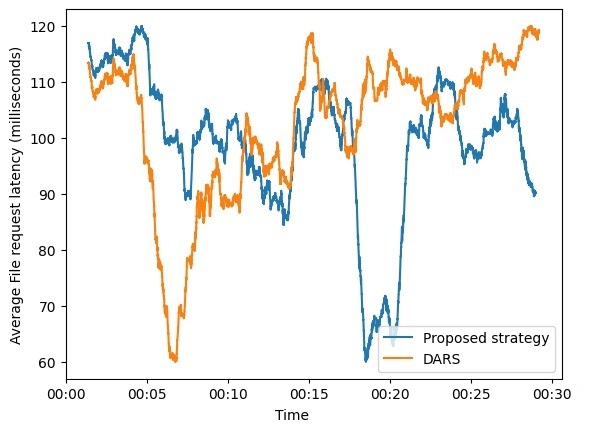
\includegraphics[width=\columnwidth]
    {project/fig/latency.jpg}
    \caption{Average file request latency of all the nodes in the network using the proposed replication strategy vs. DARS.}
    \label{fig:latency}
\end{figure}

\begin{figure}[htbp]
    \centering
    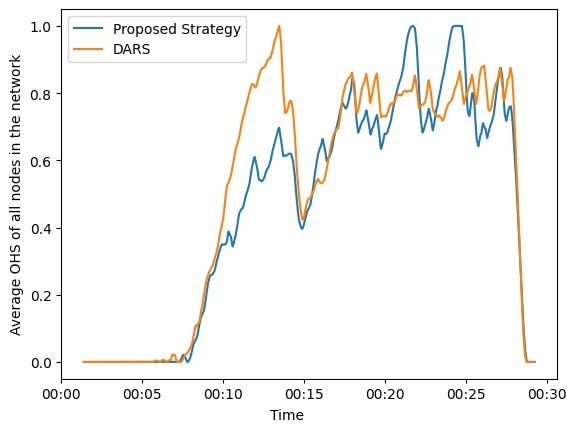
\includegraphics[width=0.45\textwidth]
    {project/fig/ohs.jpg}
    \caption{Average overheating similarity of all the nodes in the network using the proposed replication strategy vs. DARS.}
    \label{fig:ohs}
\end{figure}

\begin{figure}[htbp]
    \centering
    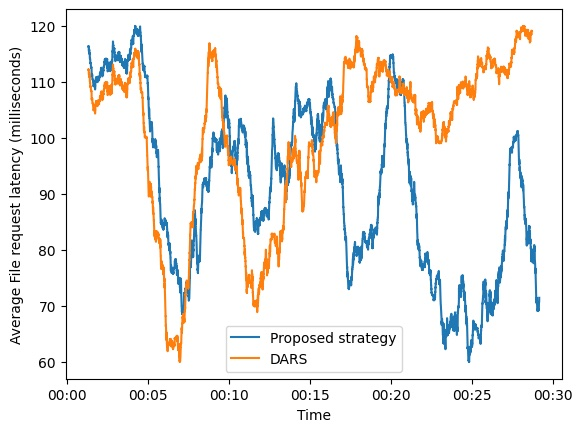
\includegraphics[width=0.45\textwidth]
    {project/fig/latency-full.jpg}
    \caption{Average file request latency of all the nodes in the network for a fully connected network topology using the proposed replication strategy vs. DARS.}
    \label{fig:latency-full}
\end{figure}

\begin{figure}[htbp]
    \centering
    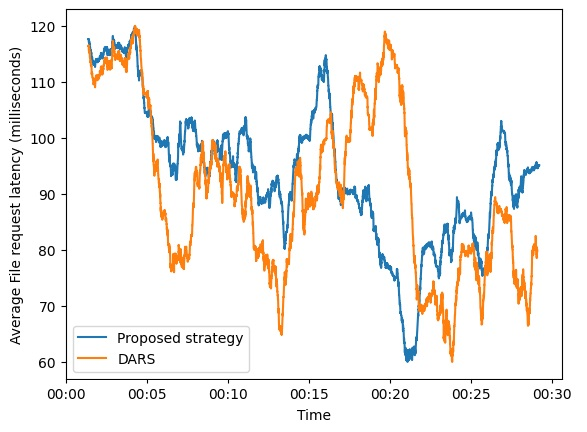
\includegraphics[width=0.45\textwidth]
    {project/fig/latency-ring.jpg}
    \caption{Average file request latency of all the nodes in the network for a ring network topology using the proposed replication strategy vs. DARS.}
    \label{fig:latency-ring}
\end{figure}

Our experiments with the proposed strategy yielded promising results. We used our P2P network simulator to run many simulations to test the efficacy of our suggested replication technique, and we compared the results to existing strategies. We assessed several primary metrics, including node availability, available bandwidth, and latency, and observed significant improvements in all of these parameters. When compared to DARS, our proposed technique resulted in higher node availability. Table \ref{tab:results} provides evidence that the proposed approach leads to significant reductions in overheat and unavailable states. It is important to note that both strategies yield different final file distributions, leading to varying levels of load balance. Consequently, the duration that a node spends in each state varies based on the final file distribution. On average, we observe a large improvement when applying our approach. However, for some individual nodes, DARS may perform better.

We attribute this improvement to the time-based file replication prioritization, which ensures that the most recently and frequently visited files are more easily available for future requests, thereby enhancing node availability. In terms of available bandwidth, the TBDF proved useful in maintaining an ideal load on each node. Our method efficiently balanced the distribution of replicas across the network by favoring recent file accesses, thereby avoiding any single node from becoming overloaded. As a result, the overall available bandwidth of the network increased. Figure \ref{fig:bandwidth} indicates that the average bandwidth utilization is lower for our proposed strategy, suggesting improved efficiency. During peak load, both DARS and our proposed strategy exhibit high bandwidth utilization. However, our strategy does not reach 100% utilization due to early optimal load balance.

We have demonstrated superior performance of our proposed technique over DARS in terms of file access latency. By strategically replicating popular files based on recent accesses, we ensured the availability of these files at neighboring nodes, effectively reducing the time required to access them and lowering the overall file access latency in the network. Figure \ref{fig:latency} clearly depicts the success of our strategy in achieving lower access latency compared to DARS. Although the average latency may initially appear higher for our proposed strategy due to additional computations, as the system load increases, it efficiently achieves optimal load balance earlier, resulting in a notable reduction in access latency.

We have observed that the proposed strategy consistently maintains a low average overheating similarity for all nodes in the network, compared to DARS, as shown in Figure \ref{fig:ohs}. This observation indicates that the risk of nodes entering an overheat condition is significantly reduced.

We also conducted experiments by changing the network topology configuration. We performed the mentioned simulations on a mesh topology (partial mesh) and analyzed the performance on both fully connected (full mesh) and ring topologies, as shown in Figure \ref{fig:latency-full} and Figure \ref{fig:latency-ring}. We observed that the proposed algorithm exhibited superior performance in the fully connected topology, while both algorithms showed comparable results in the ring topology.

In summary, we have demonstrated that our suggested algorithm significantly improves system performance, particularly in terms of node availability, available bandwidth, overheating similarity, and latency. Our findings provide strong evidence that considering the temporal locality of file accesses can greatly enhance the performance of P2P network systems.



\section{Discussion and Future Work}\label{sec:future}
Future research will concentrate on a number of relevant cloud-based peer-to-peer (P2P) system domains. It's crucial to concentrate on the duplicate replica reduction issue. While increasing the number of replicas in the system might aid in decreasing access time, it also raises the concern of increased maintenance expenses. Investigating workable techniques for getting rid of pointless clones is essential. To achieve this, it is necessary to reduce the number of replicas while maintaining strong load balancing, low access latency, and a perfect equilibrium between the replica count and system performance.

Another area that is being researched is the use of adaptive methods to fully harness the node burden for efficient replica consistency maintenance. The efficiency with which the consistency of replicas is maintained will depend on the design and implementation of approaches that can dynamically adapt to the system's diverse load scenarios. The DARS strategy's scalability in larger networks and under a wider range of conditions will also be investigated. By evaluating and enhancing the DARS method's robustness in such situations, its effectiveness can be further boosted.

\section{Conclusion}\label{sec:conclusion}

In this work, we propose a novel approach to data replication in peer-to-peer (P2P) networks using a Time-Based Decaying Function (TBDF). Our proposed strategy addresses the limitations of prior works that do not incorporate the temporal information of file requests. In our approach, we assign weights to files based on the recency of their access and progressively reduce these weights over time. To expedite the experiments, we design and implement an efficient event-driven P2P network simulator. Through simulations conducted using different network topologies and real-time trace data, we demonstrate that our approach enhances the performance and efficiency of P2P networks by significantly improving node availability, available bandwidth, and latency. Moreover, our strategy has the potential for extension and application in various distributed systems, such as content delivery networks, peer-assisted streaming systems, and high-performance computer clusters, where load balancing and efficient resource utilization are of utmost importance.



\section{Acknowledgment}\label{sec:related}
We would like to express our sincere gratitude and appreciation to Professor Haonan Wang for guiding us throughout our Master's group project. His expertise, invaluable insights, and unwavering support have played a crucial role in the successful completion of this project.
\bibliographystyle{IEEEtran}
\bibliography{IEEEmybib}

\end{document}